\section{The model, one piece at a time}\label{sec:model}

\subsection{The world in one picture}

There is a continuum of \emph{topics} and a mass $N$ of \emph{researchers}. Time is continuous and the economy is in a steady state. At any moment a researcher is in one of three situations (Figure~\ref{fig:world}): exploring at the frontier, reading her way into an existing topic, or producing inside a topic. Whenever she is free she picks the better of two options, exploring or joining, and in equilibrium the two are worth the same.

\begin{figure}[h]
\centering
\begin{tikzpicture}[font=\sffamily\small,
  box/.style={draw=axisc,line width=0.6pt,rounded corners=2pt,fill=white,align=center,inner sep=5pt,minimum height=1.25cm,text width=3.25cm},
  arr/.style={-{Stealth[length=5pt]},line width=0.8pt,color=inktwo},
  lab/.style={font=\sffamily\footnotesize,color=inktwo,align=center}]
\node[box,fill=paperc,text width=2.6cm] (free) at (0,0) {\textbf{Free researcher}\\[1pt]{\footnotesize chooses}};
\node[box] (explore) at (5.3,1.55) {\textbf{Explore}\\[1pt]{\footnotesize earns $e$ per period}};
\node[box] (found) at (10.6,1.55) {\textbf{Found a topic, stay}\\[1pt]{\footnotesize earns $v(P)$, no catch-up}};
\node[box] (catch) at (5.3,-1.55) {\textbf{Join: catch up}\\[1pt]{\footnotesize reads the stock for $T(P)$ years, earns nothing}};
\node[box] (prod) at (10.6,-1.55) {\textbf{Produce}\\[1pt]{\footnotesize earns $v(P)$ as an incumbent}};
\draw[arr] (free.north east) -- node[lab,above left=-1pt and 0pt] {value $F$} (explore.west);
\draw[arr] (free.south east) -- node[lab,below left=-1pt and 0pt] {value $w(P)$} (catch.west);
\draw[arr] (explore) -- node[lab,above] {rate $s$} (found);
\draw[arr] (catch) -- node[lab,above] {after $T(P)$} (prod);
\node[lab,color=hbluedark] at (5.3,0) {\textbf{Equilibrium:}\quad $w(P^*)=F$};
\end{tikzpicture}
\caption{A researcher's options. Every spell ends at rate $\rho$ (her career in that topic ends) or $\xi$ (the topic becomes obsolete), and she is then free again. Payoffs are per unit of production speed $a$.}
\label{fig:world}
\end{figure}

Six objects carry the whole model.

\begin{center}\small
\begin{tabularx}{\textwidth}{@{}P{0.55in}P{1.6in}L@{}}
\toprule
Symbol & Name & Meaning \\
\midrule
$a$, $b$ & production and reading speed & Projects produced, and papers read, per year of full-time work. \\
$P$ & density & The flow of papers a topic produces per year. The measure of crowding. \\
$v(P)$ & payoff curve & What an incumbent earns per period in a topic of density $P$, per unit of $a$. \\
$w(P)$ & newcomer's payoff & What a newcomer earns on average over her spell: $v(P)$ scaled down by the time she spends catching up. \\
$F$ & frontier value & What exploring is worth per period. \\
$\EE$ & volume elasticity & By how much density rises when the number of researchers rises by 1\%. \\
\bottomrule
\end{tabularx}
\end{center}

\subsection{Inside a topic: the two jobs of reading}

\subsubsection{Time, production and density}
A researcher has one unit of time per period. She spends a share $x$ producing and a share $r=1-x$ reading. Full-time production yields $a$ projects per period; full-time reading covers $b$ papers. A topic with $n$ producing members therefore receives a flow of
\[
P = a\,x\,n \quad\text{papers per period.}
\]
This flow is the topic's \emph{density}. The paper is explicit that $a$ is research output per unit of production time (doing the research and writing it up), not drafting speed: a tool that drafts text faster raises $a$ only by the share of production time that drafting takes.

Density is a flow. What a researcher learns from, and what can pre-empt her project, is the topic's current literature. What a newcomer must master is the \emph{stock}, the accumulated literature. The distinction is the one between keeping up with a field and getting into it, and it matters only for topics that grow or shrink.

\subsubsection{Job one: reading teaches}
Reading a share $r$ of the time covers $R=br$ papers of the topic's flow. What she reads raises the quality of her own work by a factor $Q(R,P)\ge 1$. The paper assumes (Assumption~1) that nothing is learned without reading or without a literature, that what one can learn is bounded by what one reads, and that $\ln Q$ is jointly concave and supermodular: no increasing returns to reading, and reading is worth more where there is more to read. The running example is
\[
Q(R,P)=\bigl(1+\beta\,h(R,P)\bigr)^{\gamma},\qquad h(R,P)=\frac{RP}{R+P},
\]
where $h$ is close to $R$ when she samples a small part of a rich literature and close to $P$ when she reads a thin one exhaustively.

\subsubsection{Job two: reading protects}
Each earlier paper in the topic \emph{covers} her project with a small probability, so the number of earlier covering papers is Poisson with mean $\theta P$. She catches a covering paper only if she finds it. With reading coverage $c=R/P$ this happens with probability $\varphi(c)$, increasing and concave (Assumption~2); the example is $\varphi(c)=1-e^{-\sigma c}$, where $\sigma$ is search precision. Some overlap cannot be prevented: projects in progress elsewhere arrive at rate $\theta_cP$ and cannot be found in the literature.

Overlap erodes credit. An undetected earlier covering paper removes a share $\lambda$ of the project's credit; a concurrent one removes $\lambda_c$. If she catches a covering paper she either \emph{pivots} to a fresh variant (keeping $1-\kappa_p$) or \emph{proceeds} as a follow-on that cites the earlier paper (keeping a random share $\delta$). She loses $\ell<\lambda$ on average after a detection, so detection is worth $\Delta=\lambda-\ell$.

\begin{resultbox}{Lemma 1}{Credit and overlap}{\tminor}
Expected credit per project is
\[
C(R,P)=\exp\Bigl\{-\theta P\bigl[\lambda-\Delta\,\varphi(R/P)\bigr]-\theta_c\lambda_cP\Bigr\}.
\]
Earlier covering papers that the researcher does not pivot away from (``flagged overlap'') arrive at rate $\theta P[1-(1-q)\varphi]$, where $q$ is the share of detections that proceed. A share $A=q\varphi/[1-(1-q)\varphi]$ of them is \emph{aware}: the later paper cites the earlier one.
\tcblower
\inwords Credit falls exponentially with the number of papers in the topic, and reading slows the fall. The formula also says what the data should show: how often a paper sits very close to an earlier one, and how often it cites it.

\role It connects the model to two observables (the overlap rate and the aware share) and supplies the falling arm of the payoff curve. The paper says that its incidence results do not depend on it.

\review Correct. But the block is quantitatively inert (overlap destroys 2.9\% of credit at the calibrated density), it absorbs most of the paper's empirical effort, and its inputs are soft (\S\ref{sec:crit-evidence}).
\end{resultbox}

\subsubsection{The researcher's problem and the payoff curve}
A researcher in a topic of density $P$ earns $a\,x\,Q\,C$ per period. Dividing by $a$:
\[
g(r,P)=(1-r)\,Q(br,P)\,C(br,P),\qquad v(P)=\max_{r\in[0,1)} g(r,P).
\]
The function $v$ is the \emph{payoff curve}. Production speed scales every payoff and drops out of it. The researcher takes $P$ as given: she ignores that her papers teach her colleagues and that they add to what her colleagues must read.

\begin{resultbox}{Theorem 1}{The payoff curve}{\tsolid}
For any learning and detection technology satisfying the assumptions above:
(i)~$v(0)=1$ and $v(P)\to0$ as $P\to\infty$;
(ii)~$\ln v$ is concave;
(iii)~$v$ rises up to a unique peak $\Phat$ and falls afterwards, with $v(\Phat)>1$;
(iv)~its slope is
\[
\frac{v'(P)}{v(P)}=\underbrace{\partial_P\ln Q}_{\text{more to learn from}}-\underbrace{\theta\bigl[\lambda-\Delta\bigl(\varphi(c^*)-c^*\varphi'(c^*)\bigr)\bigr]-\theta_c\lambda_c}_{\text{more to miss}};
\]
(v)~the optimal reading share $r^*(P)$ rises with density, so papers per researcher fall with density.
\tcblower
\inwords A thin topic gets better as it fills, because there is more to learn from. A crowded topic gets worse as it fills, because more of what you do has already been done and you cannot read it all. In between there is one best size.

\why $\ln g$ is jointly concave in reading time and density. The erosion term is linear in $P$ plus the perspective of the concave function $\varphi$, and perspectives preserve concavity. Maximising a jointly concave function over one argument leaves a concave function of the other. The fall comes from \emph{bounded absorption}: what one person can read and learn is bounded, while the number of papers that may cover her project grows in proportion to the literature.

\review The proof was rederived and holds. Two caveats on its use. The calibrated curve is nearly flat: $v$ lies between 1.78 and 1.98 for densities from 2 to 39 papers a year. And part~(v) has the wrong sign in the data: papers per author rise by 0.5\% per standard deviation of density, where the calibrated model implies a fall of 1.3\%.
\end{resultbox}

\begin{figure}[h]
\centering
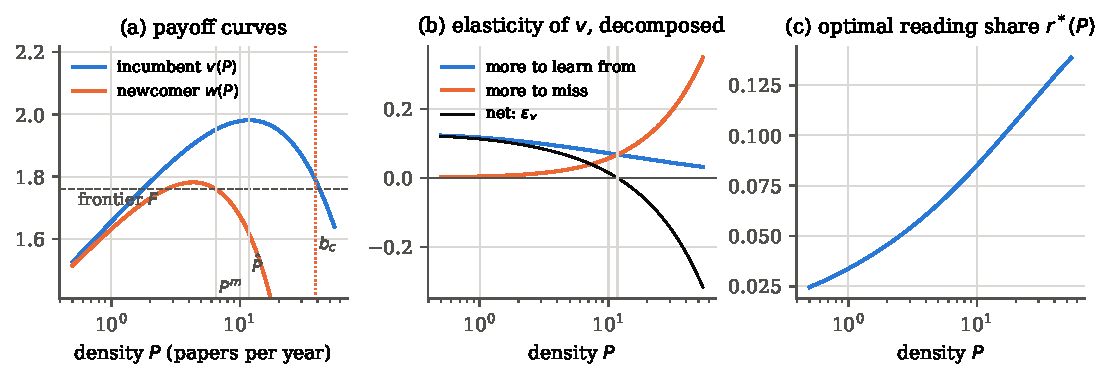
\includegraphics[width=0.98\textwidth]{fig1_payoff_curve.pdf}
\caption{From the paper (its Figure~1). Left: the payoff curve $v(P)$ and the newcomer's payoff $w(P)$ in the calibrated model, with the peak $\Phat$, the mature density $\Pm$ where $w=F$, and the speed limit $b_c$ where $w$ vanishes. Right: the two forces in the slope of $v$ and the optimal reading share.}
\label{fig:payoff}
\end{figure}

\begin{resultbox}{Lemma 5}{Time shares}{\tsolid}
At a given density, $\partial\ln v/\partial\ln b=r^*/(1-r^*)$, and a faster production speed raises the payoff one for one. A speed-up of a task that takes a share $s_k$ of her time saves $s_k\,\dd\ln(\text{speed})$ of her time and raises her payoff by that amount divided by $x^*$. Per unit of time saved, every speed-up is worth the same.
\tcblower
\inwords Inside a topic a tool is worth the time it saves. Reading takes about 7\% of an incumbent's time and production the rest. So a tool that makes reading 30\% faster is worth about 2 log points, and one that makes production 30\% faster is worth 26. Per hour saved they are worth the same.

\why Two lines: the envelope theorem and the first-order condition for reading.

\review Solid, and it does real work: it shows that the old ``writing beats reading'' comparison was mostly about time shares. One caveat: the 7\% comes from a survey of all reading by all faculty and is matched to producing incumbents only. Counting the full-time reading that the model requires of newcomers, reading is 15.8\% of topic members' time (\S\ref{sec:crit-calib}).
\end{resultbox}

\begin{resultbox}{Proposition 1}{The sign of the spillover}{\tsolid}
One more paper in a topic of density $P$ changes each incumbent's payoff by $a\,v'(P)$: positive below the peak, negative above it.
\tcblower
\inwords Whether an extra paper helps or hurts its neighbours is derived, not assumed. It depends on where the topic sits on its payoff curve.
\end{resultbox}

\subsection{Getting into a topic: catch-up}\label{sec:model-catchup}

Careers in a topic end at rate $\rho$, and topics become obsolete at rate $\xi$. The literature a newcomer must master is a stock $S$ that accumulates the flow and loses relevance at rate $\delta$:
\[
\dot S=P-\delta S,\qquad\text{so } S=P/\delta \text{ in a stationary topic.}
\]
She reads it at speed $b_c$ before she can contribute. Papers that appear while she reads must be read too, so her backlog $B$ follows $\dot B=P-\delta B-b_c$ from $B(0)=S$. This is a topic-level version of the ``burden of knowledge'' of Jones (2009).

\begin{resultbox}{Lemma 2}{Catch-up and the speed limit}{\tsolid}
With a constant flow $P$ and an initial stock $S$, catch-up takes
\[
T(P,S)=\frac1\delta\ln\Bigl(1+\frac{\delta S}{b_c-P}\Bigr)\ \text{ if } P<b_c,\qquad T=\infty\ \text{ if } P\ge b_c .
\]
A newcomer to a stationary topic earns on average over her spell
\[
w(P)=v(P)\,\Gamma(P),\qquad \Gamma(P)=e^{-(\rho+\xi)T(P)}=\Bigl(1-\frac{P}{b_c}\Bigr)^{\nu},\qquad \nu=\frac{\rho+\xi}{\delta}.
\]
A share $(1-P/b_c)^{\rho/\delta}$ of a stationary topic's members have caught up and produce.
\tcblower
\inwords Catching up is a race between the reader and the literature. The time it takes rises more than in proportion to the flow, and it is infinite once the literature grows as fast as she reads. Incumbents earn $v$; a newcomer earns $w<v$ because part of her spell goes into reading. Catch-up reading buys admission and nothing else.

\review The formula is right, and it is a real improvement on the linear cost of the previous version. The \emph{limit} it implies depends on an admission standard that incumbents do not meet (\S\ref{sec:crit-speed}). The last sentence, the count of who is producing, is the one that later contradicts Lemma~4 (\S\ref{sec:crit-lemma4}).
\end{resultbox}

\subsection{The frontier}

Instead of joining a topic a researcher can explore. An explorer produces $e$ per period (exploratory work that founds nothing lasting) and founds a viable topic at rate $s$. \emph{A founder stays} in the topic she opens: she wrote its first papers, needs no catch-up, and remains an incumbent until her career there ends or the topic dies. Topics are born at rate $sE$, where $E$ is the number of explorers, and die at rate $\xi$. In a steady state births equal deaths, $sE=\xi M$, where $M$ is the number of open topics.

\begin{resultbox}{Lemma 3}{The value of the frontier}{\tsolid}
The value of exploring per period is
\[
F=(1-\omega)\,e+\omega\,\bar U_F,\qquad \omega=\frac{s}{\rho+\xi+s},
\]
where $\bar U_F$ is the founder's average payoff over the life of the topic she opens. The share of this value that founders earn as incumbents is
\[
\thF=\frac{\omega\,\bar U_F}{F}\in[0,1).
\]
The frontier is depleted as more topics are opened: $F$ falls with the number of open topics at elasticity $\etaF\ge0$.
\tcblower
\inwords Exploring pays in two ways: what you produce while you look, and what you earn as the first insider of the topic you find. $\thF$ is the weight of the second. It is the statistic on which the paper's incidence result turns, and nothing in the paper measures it.

\review The algebra is right. In the stationary economy the paper sets $\bar U_F=v(P)$, as if a newborn topic had its mature density at once. On the paper's own life-cycle simulation founders live mostly through the growth phase and earn 1.82, not 1.95 (\S\ref{sec:crit-founders}). And $\omega$ is the share of time spent as a founder, not a probability as the notation table says.
\end{resultbox}

\begin{resultbox}{Lemma 4}{Output equals the frontier}{\trepair}
In a stationary equilibrium in which every option a free researcher takes is worth $F$, output per researcher is exactly $aF$: \quad $Y=a\,N\,F$.
\tcblower
\inwords If everyone is always indifferent between her options and exploring, then on average everyone earns what exploring is worth. Every question about long-run productivity becomes a question about the frontier.

\why The renewal-reward theorem: a researcher's long-run output per period is the common value of the spells she moves through.

\review This is the step that fails. Its premise does not hold in the economy the paper defines: some members never paid the entry cost. With the member count of Lemma~2, output per researcher is $aF\,e^{\xi T}$, 1.2--3.0\% above $aF$, and the headline numbers change (\S\ref{sec:crit-lemma4}).
\end{resultbox}

\subsection{Equilibrium}

\begin{resultbox}{Definition 1}{Topic equilibrium}{}
A density $P^*$ for every open topic, a production share $x^*$, a number of open topics $M^*$ and a number of explorers $E^*$ such that:
(i)~researchers split their time optimally, $x^*=x^*(P^*)$;
(ii)~newcomers are indifferent between joining and exploring, $w(P^*)=F(M^*,P^*)$;
(iii)~the allocation is stable under entry, $w'(P^*)<0$;
(iv)~births equal deaths and researchers add up, $sE^*=\xi M^*$ and $E^*+M^*n(P^*)=N$.
\tcblower
\inwords Topics fill until joining one is worth no more than opening one. Stability requires that the crossing is on the falling side of the newcomer's payoff: where $w$ still rises, one more entrant makes entry more attractive and draws in more.

The comparative statics are stated in the \emph{large-topic limit}, in which explorers are few relative to topic members, so $M^*\approx N/n(P^*)$.
\end{resultbox}

\begin{keybox}[The model in four sentences]
Inside a topic, more papers first help (more to learn from) and then hurt (more to miss): the payoff curve $v(P)$ has one peak.
Getting into a topic costs reading time that grows with its literature, so newcomers earn $w(P)<v(P)$ and insiders keep the difference.
Outside the topics there is a frontier worth $F$, where people look for new topics and stay in the ones they find.
Topics fill until $w(P^*)=F$.
\end{keybox}
